\chapter{Descripción del Trabajo}
\label{cap:descripcionTrabajo}

%En este capítulo abordaremos los aspectos tanto de diseño como de implementación de nuestra aplicación...TO BE CONTINUED

\section{Reunión en el Centro de Tiflotecnología e Innovación de la ONCE}

La idea de este TFG surge de la necesidad de resolver problemas reales para gente real, concretamente para personas con discapacidad visual. De esta manera, empezamos nuestro camino por lo más importante: conocer las necesidades de los usuarios finales. Con este fin y gracias a la oportunidad que nos ha brindado la Universidad Complutense de Madrid con la profesora María Guijarro al frente, hemos podido reunirnos y entrevistar a personas especializadas en el campo de las tecnologías que sufren discapacidad visual.

En este documento recogemos las notas que tomamos durante la reunión el pasado 11 de octubre de 2019 en el CTI (Centro de Tiflotecnología e Innovación) de la ONCE.
	

%PRIMERA SECCIÓN
\subsection{Introducción}
La entrevista comenzó con una breve explicación, de la mano de José María Ortiz, director del Departamento de Consultoría e Innovación, sobre las principales tareas que se llevan a cabo en el centro, entre las cuales destacan:

\begin{itemize}
	\item Ayudar a una persona con discapacidad visual en su \textbf{adaptación} al trabajo y a la vida cotidiana, proporcionandole para ello el material necesario (teclados, líneas de braille, bastones, etc.).
	\item Responder a \textbf{consultas} sobre el funcionamiento de dispositivos.
\end{itemize}

Luego, nos comentó los departamentos en los que se estructura el centro para que pudiésemos hacernos una idea más global de todo lo que abarca. Éstos son:

\begin{itemize}
	\item \textbf{El departamento de Consultoría e Innovación:} donde actualmente están desarrollando el programa EDICO en colaboración con la UCM, que tiene como objetivo hacer las matemáticas accesibles mediante un editor de texto. De manera paralela se encargan del desarrollo de aplicaciones de muy diversa índole, véase apps para la biblioteca de la ONCE, de películas audio-descritas, etc.
	\item \textbf{Departamento de Evaluaciones y Auditoría:} donde se encargan de evaluar los productos que se van a sacar al mercado.
	\item \textbf{Departamento de diseño y producción:} donde se encargan de, tal y como indica su nombre, diseñar y producir elementos de adaptabilidad, como pueden ser unas plantillas con relieve de policarbonato para las vitrocerámicas. Recordemos que estas, aunque no presentan dificultad alguna para los usuarios videntes, son tediosas para aquellos que cuentan con discapacidad visual ya que la pantalla táctil no tienen ningún tipo de relieve que pueda servirles como referencia y guiarles en su uso.
	\item \textbf{Departamento de Asesoría en tecnología:} especializado en tecnologías accesibles.
\end{itemize}

Una vez concluida esta sección en la que nos contextualizaron, abrieron paso a la ronda de preguntas en la que pudimos acercarnos a ellos, conociendo sus problemas y necesidades en el día a día.

%SEGUNDA SECCIÓN
\subsection{Entrevista}

Durante esta parte, nos dirigimos especialmente a Mónica y José Luis Llorente, ambos ingenieros del CTI, para que, con su experiencia y conocimientos, nos explicaran lo máximo posible sobre tecnologías accesibles y nos dieran su punto de vista en las ideas que proponíamos. Por otro lado, Mónica no solo era experta en la materia sino que además era invidente, por lo que nos pudo contar su perspectiva y necesidades como usuaria.

Las preguntas avanzaron desde temas generales para conocer cómo una persona invidente se desenvuelve con la tecnología, sus gustos y qué sensaciones le despierta, hasta temas concretos dirigidos a conocer los problemas que plantea la navegación por espacios interiores.

\begin{itemize}
	\item  \textbf{¿Cómo utiliza una persona con discapacidad visual un dispositivo móvil?}
	
	Para responder a esta pregunta, Mónica nos hace una demostración en directo, para ello emplea un móvil Xiaomi con sistema operativo Android.
	
	Mónica nos cuenta que para la navegación por su dispositivo utiliza un lector de pantalla, es decir, un software que facilita el uso del sistema operativo. Éste sirve como guía para las personas que, como ella, tienen discapacidad visual, ya que ``lee y explica'' mediante voz lo que se ve en la pantalla. Los lectores de pantalla vienen siempre incluidos en el dispositivo y se pueden encontrar en la sección de Accesibilidad, en Ajustes. En el caso de Android, este software se llama \textit{Talkback} y es configurable. Por ejemplo, dice Mónica, se podría usar mediante la línea de braille en vez de la reproducción por voz.
	
	Luego vemos como se desplaza por las aplicaciones utilizando \textit{flicks}, movimientos secos en los que desliza el dedo hacia uno de los lados de la pantalla (izquierda o derecha, según interese). Del mismo modo, para la navegación por la web o dentro de alguna aplicación utiliza estos movimientos hacia arriba y hacia abajo. Por último, nos muestra cómo accede a un elemento mediante doble click. 

	También nos habla de la posibilidad de la navegación libre, eso sí, solo cuando ya te has familiarizado con el dispositivo lo suficiente como para saber dónde tienes determinadas aplicaciones. 

	Lo más cansado, según Mónica, es tener que hacer un barrido por toda la pantalla hasta encontrar lo que quieres, en vez de poder ir directamente. Para agilizar un poco este proceso, Mónica, por ejemplo, agrupa las aplicaciones por carpetas, de modo que el barrido es más sencillo que si la pantalla estuviese repleta.
	
	Para las personas con baja visión también existe la posibilidad de hacer más grandes los iconos y ajustar los colores.
	
	% Segunda pregunta:
	\item \textbf{Hemos leído que normalmente las aplicaciones se desarrollan para dispositivos iOS, ¿por qué es mejor?} 
	
	\textit{``Si que es cierto que solía ser así ya que iOS le llevaba la delantera a Android en cuanto a accesibilidad, pero cada vez se usa más Android pues las diferencias están completamente recortadas, están muy igualados y los precios son mucho más asequibles. Yo misma, antes tenía un iPhone y ahora me he pasado a Android y no hay nada que eche en falta.''}, responde Mónica.
	
	% Tercera pregunta:
	\item \textbf{¿Cómo afronta una persona ciega su desplazamiento y orientación por interiores cuando pisa por primera vez dicho espacio u edificio?}
	
	Ante esta pregunta Mónica resopla y nos contesta: \textit{``Buufff..., ¿te vale?''}
	
	Nos puso como ejemplo la llegada a un hospital: \textit{``cuando entras necesitas saber, al menos, dónde está la recepción para pedir ayuda pero los carteles informativos están fuera de mi alcance, entonces entro por la puerta y pienso ¿y ahora qué?. ¿Dónde está el mostrador de recepción? No es tan fácil como echar un primer vistazo, necesitas ayuda mediante voz, algo que te describa el espacio y te vaya diciendo que hay a derecha e izquierda y a cuantos metros.''}

	Nos contó que en cuanto a la descripción/guía por espacios interiores ahora mismo no hay disponible ninguna aplicación. Por ello, una vez superada la primera barrera de ubicar y localizar un cierto destino, la única opción que les queda es la de memorizar el camino. Mónica destacó que era increíble la cantidad de rutas que tiene en la cabeza.
	
	Por todo esto, se comentó que una aplicación sería de gran ayuda para ellos, de manera que pudiesen tener una idea del edificio incluso antes de llegar a él para moverse con más seguridad. Una app que no solo les guiase a un punto concreto, sino que además describiese el edificio, indicándoles qué posibilidades les ofrece. También se mencionaron otras propuestas e ideas como tener previamente el plano del edificio para poder ir moviéndote con el dedo sobre él y que a su paso te vaya indicando las distintas salas que aparecen, o la impresión de un mapa 3D que disponga de un código QR o algo similar que fuese capturado mejor por Bluetooth que por foto que tras leerlo cargase el plano del edificio y pudiese proporcionar tanto información sobre el espacio en sí mismo (número de plantas, qué hay en cada una...) como información más precisa como puede ser averías, horarios, disponibilidad de salas, etc.
	 
	Obviamente de la mano de estas ideas surgían problemas y opiniones en contra: ¿Dónde estaría dicho mapa?, ¿Cómo encontrarlo?, ¿Todos los edificios estarán de acuerdo en facilitar los planos o puede que por motivos de seguridad no sea una idea factible?, ¿es posible llegar a un standard para que se pueda usar el mismo sistema en cualquier edificio?
	
	% Cuarta pregunta:
	\item \textbf{¿Hay algún tipo de señales que os sirvan como referencia a la hora de desplazaros por un edificio?}
	
	\textit{``Hay señales de encaminamiento, que te indican dónde están las escaleras, ascensores, zonas de cruce, etc.''}, contesta.

	% Quinta pregunta:
	\item \textbf{¿Cuántos edificios cuentan con estas señales?}
	
	\textit{``La verdad que cada vez son más frecuentes y hoy en día se encuentran en casi todos los edificios, especialmente en los nuevos.''}, responde.
	
	% Sexta pregunta:
	\item \textbf{¿Cómo de factible es ir con el dispositivo móvil en la mano, para realizar una foto o cualquier cosa similar?}
	
	\textit{``Puedo hacer una foto en un momento puntual, en eso no hay problema alguno pero no es cómodo ir con el móvil en la mano constantemente porque además de que es aparatoso porque ya llevo en la mano el bastón, perro guía, etc. No es práctico, no sería la primera vez que roban un móvil a una persona invidente, es una realidad.''}, contesta Mónica. \textit{``Particularmente, con respecto a la foto el problema principal sería saber a dónde enforcar''}, añade.
	
\end{itemize}

%Creo que es mejor subsection para las conclusiones del TIC
%TERCERA SECCIÓN
\subsection{Conclusiones}
Tras el debate, algunas de las conclusiones que sacamos de la visita al CTI son:

\begin{itemize}
	\item La implementación de una aplicación como la nuestra es muy útil y necesaria.
	\item Las modalidades más empleadas para interactuar con el móvil cuando tienes algún tipo de rastro visual son: flicks, sacudidas, mediante vibración, arrastrando o pulsando la pantalla con un dedo, dos,...
	\item No resulta cómodo ir barriendo el espacio con la cámara del móvil.
	\item El uso de dispositivos adicionales como una micro cámara, en principio, no sería un problema, siempre y cuando no la tengan que llevar de manera continuada en la mano.
	\item En caso de auriculares, se recomienda utilizar auriculares óseos de modo que dejen el canal auditivo libre para captar otros estímulos.
	\item El objetivo es que el grueso de las aplicaciones sean lo más inclusivas posibles, es decir, que su uso sea apto tanto para personas videntes como invidentes.
	\item El feedback de la aplicación no debe saturar pero sí se aconseja que sea constante para que no se malinterprete que la aplicación ha dejado de funcionar.
\end{itemize}


\section{Estudio de la precisión de los beacons}

Antes de embarcarnos en el diseño de la aplicación vamos a hacer un estudio más en profundidad de los \textit{beacons} con el fin de comprender por completo su funcionamiento y cómo se comportan a la hora de medir distancias, es decir, cuánto rango tiene la señal \textit{bluetooth}, con ayuda de qué función podemos recibir esta señal e interpretarla para determinar la distancia, qué margen de error presenta, en qué lugares es más aconsejable establecer las balizas para recibir mejor la señal y por tanto reducir el error, etc. % REFERENCIA AL PDF DE WAYFNDER.

Los \textit{beacons} utilizados para este proyecto cuentan con una SDK (Kit de Desarrollo Software) propia de su marca (\textit{Kontakt}) en la que incluyen funciones ya implementadas que nos permiten conocer qué \textit{beacons} están en nuestro rango en un momento determinado y a cuántos metros están, y se va actualizando cada cierto tiempo. También incluye un sistema de categorías en función de cómo de cerca o lejos esté un cierto dispositivo. Las categorías son las siguientes:

\begin{itemize}
	\item \textit{IMMEDIATE:} Si el dispositivo se encuentra a menos de $0,5$ metros.
	\item \textit{NEAR:} Si el dispositivo se encuentra entre $0,5$ y $3$ metros.
	\item \textit{FAR:} Si el dispositivo se encuentra a más de $3$ metros.
	\item \textit{UNKNOWN:} Si se ha perdido la señal del dispositivo.
\end{itemize}

Gracias a estas funciones hemos desarrollado una serie de aplicaciones que nos han servido para tener una primera toma de contacto con el entorno de programación que hemos escogido, Android Studio, y para contrastar de manera visual el error existente entre la distancia real a la que se encuentran las balizas y la distancia leída mediante la interpretación de las señales bluetooth. Las aplicaciones son las siguientes:

%Android no es un lenguaje de programación, es el SO. He puesto el entorno Android Studio, si no te cuadra podemos poner otra cosa

\subsection{Aplicación \textit{miniapp}}
Esta aplicación constituye la primera toma de contacto con los \textit{beacons} y con el código de la SDK. Presenta una interfaz sencilla en la que aparece una tabla con las distintas categorías de proximidad para 3 balizas y, debajo, el hueco para indicar el identificador correspondiente. En el cuadro inferior aparecen dos botones muy intuitivos con los que el usuario puede interactuar con la app: Stop Scanning y Start Scanning. De esta manera, una vez que empieza el escaneo y las balizas se encuentran en el radio de detección, se incluyen los identificadores en cuestión y se colorea en verde la categoría de proximidad estimada en cada caso según corresponda. La lectura de los \textit{beacons} se actualiza cada 2 segundos, tiempo establecido de antemano. En la Figura \ref{fig:miniapp} podemos ver la interfaz descrita.

La idea subyacente para desarrollar esta aplicación es la de establecer el grado de confianza que podemos tener en las categorías ofrecidas por la SDK de \textit{Kontakt} y así, ver si podemos reutilizarlas para dar ciertas instrucciones al usuario cuando este se encuentre en un cierto rango. %El resultado ha sido muy positivo puesto que, a pesar de que las distancias en metros sí fluctuan, la categoría asignada se corresponde en líneas generales con la real. 

\begin{figure}[t]
	\centering
	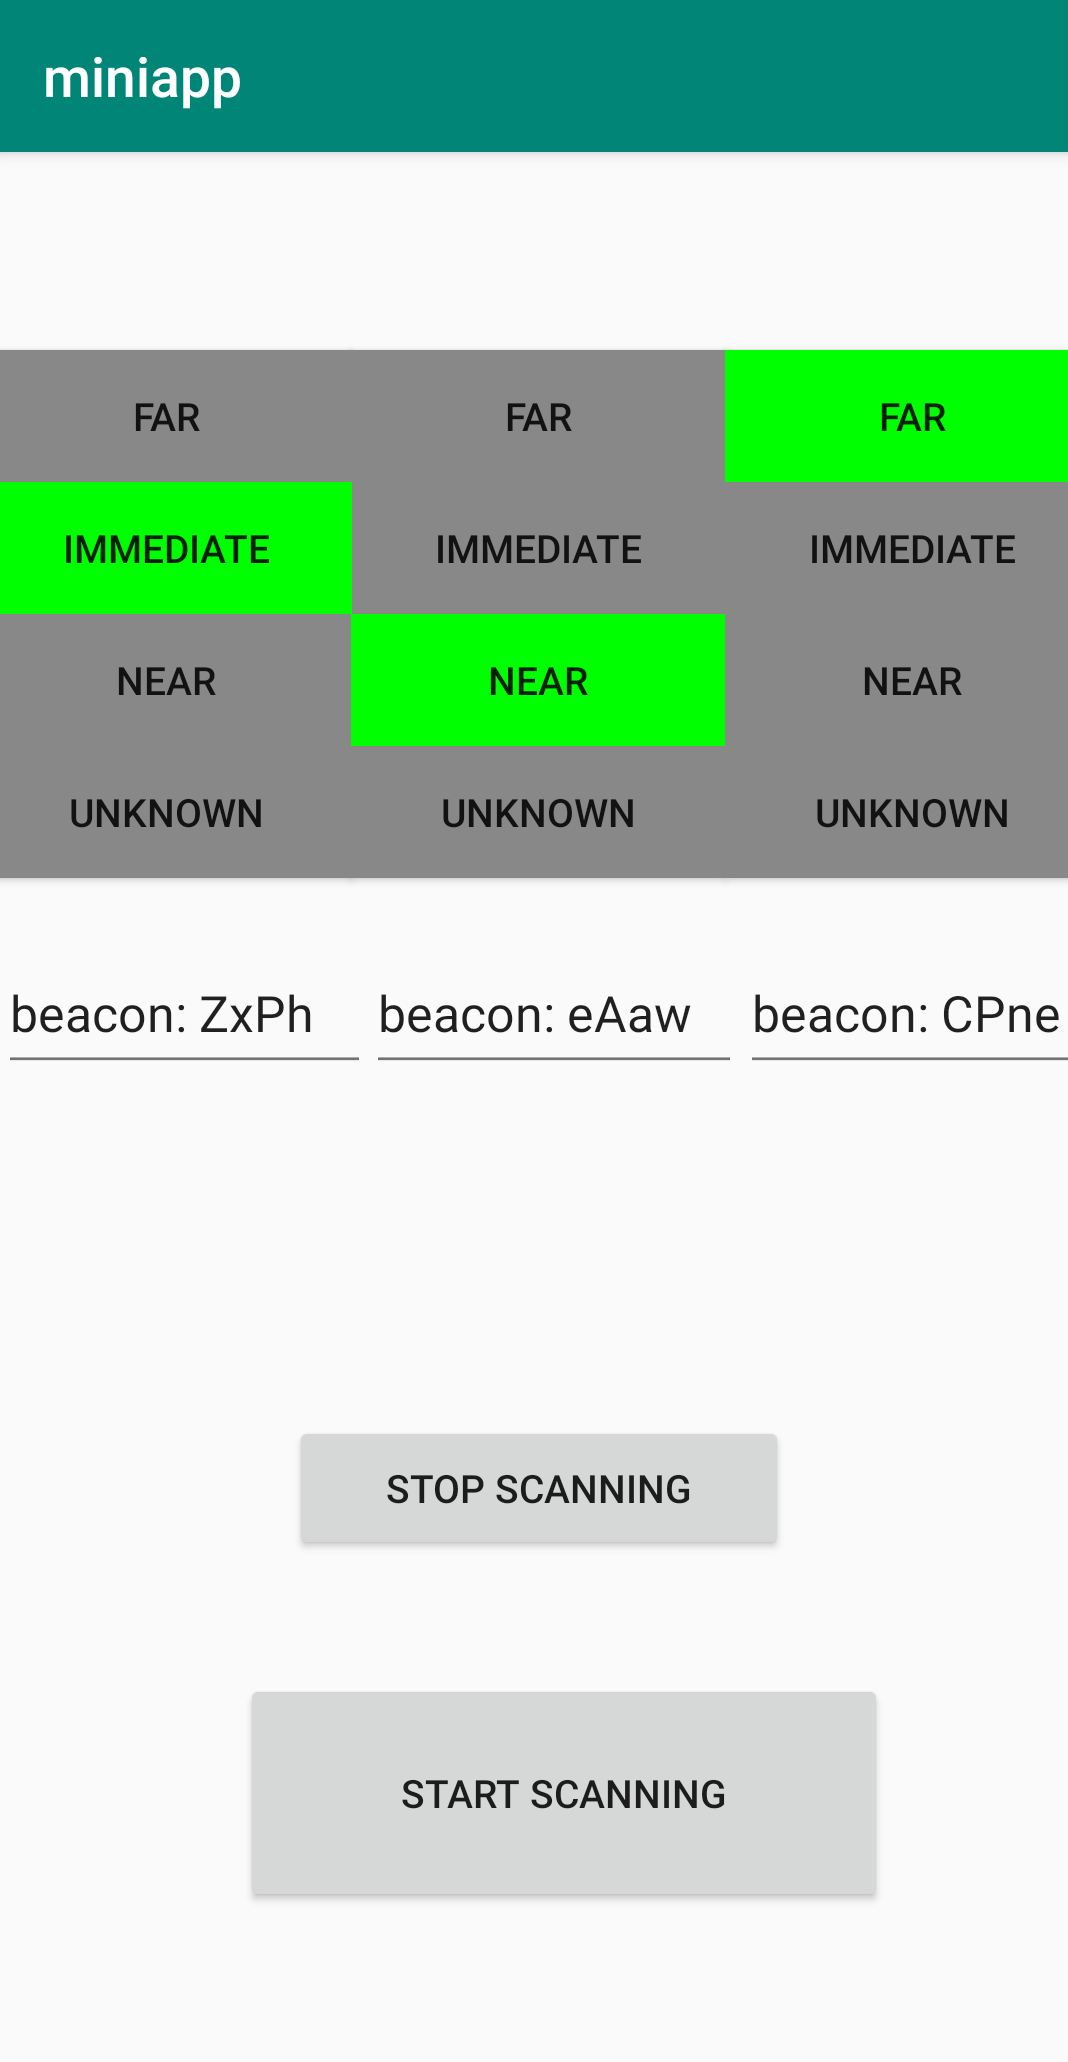
\includegraphics[width=0.4\textwidth]{Imagenes/Descripciondeltrabajo/miniapp}
	\caption{Interfaz de la aplicación miniapp. }
	\label{fig:miniapp}
\end{figure}

\subsection{Aplicación \textit{cuadrantes v1}}
Tras la aplicación \textit{miniapp}, hemos desarrollado una segunda, llamada \textit{cuadrantes v1}, capaz de captar los \textit{beacons} al paso e indicar la categoría de proximidad y los metros exactos a los que lee las balizas. Esta información se actualiza cada 2 segundos (tiempo configurable). La Figura \ref{fig:cuadrantesv1} muestra la interfaz principal de la aplicación.

La idea por la cual hemos creado la app \textit{cuadrantes v1} es la de obtener más información sobre el error cometido a la hora de determinar la distancia en metros a la que se encuentran los \textit{beacons} y ver qué factores le afectan para poder empezar a pensar los puntos claves en los que colocar las balizas y abordar, tras ello, el mapeo de la edificio. De ahí el nombre de la aplicación ya que, como veremos, los cuadrantes serán una pieza fundamental en el mapeo.

\begin{figure}[t]
	\centering
	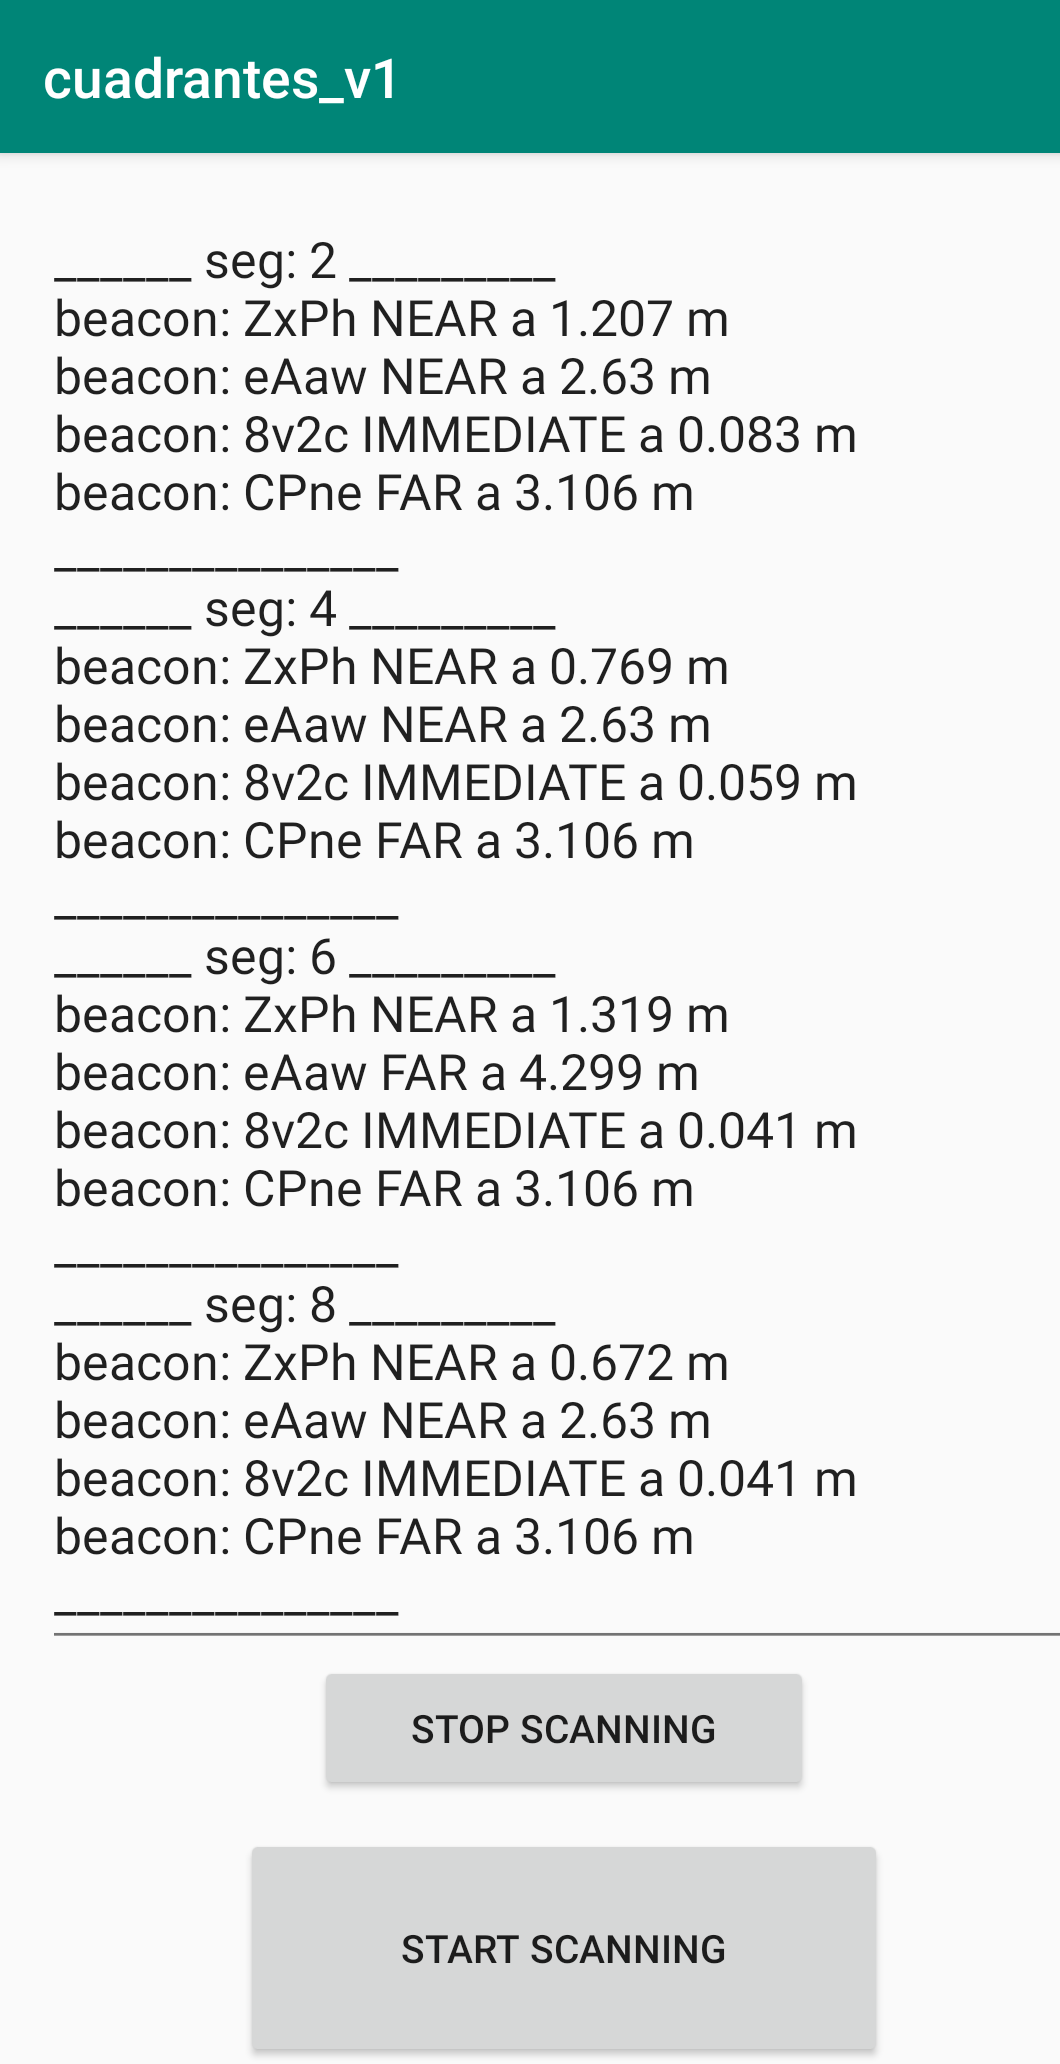
\includegraphics[width=0.4\textwidth]{Imagenes/Descripciondeltrabajo/cuadrantes_v1}
	\caption{Interfaz de la aplicación cuadrantes v1.}
	\label{fig:cuadrantesv1}
\end{figure}


\subsection{Resultados}

A continuación presentaremos algunos de los resultados obtenidos en las distintas mediciones realizadas. Para ello, hemos creado unas gráficas que muestran cómo se comportan los \textit{beacons} si comparamos la medida real con la estimada por la aplicación. 

En la Figura \ref{fig:dist_CPne} vemos las lecturas que nos ha proporcionado la aplicación \textit{cuadrantes v1} del \textit{beacon} con identificador CPne. En este caso, hemos realizado 4 estudios independientes marcados con distintos colores: azul -\textit{beacon} a 2m-, naranja -\textit{beacon} a 2,5m aproximadamente-, gris -\textit{beacon} a 5 metros- y amarillo -\textit{beacon} a 64cm-. De esta gráfica concluimos que cuanto mayor es la distancia a la que se encuentra la baliza, véase la función grisácea (5m), más fluctúa la medida estimada convirtiéndose en un dato poco fiable. Correlativamente, a menor distancia menor error. Podemos ver que la función azul (2m) es bastante fiel a la realidad, fluctúa en un intervalo de un metro a lo largo de toda la medición. Por último, el resultado de la gráfica amarilla (64cm) es bastante preciso, presenta un error despreciable durante toda la medición.

\begin{figure}[t]
	\centering
	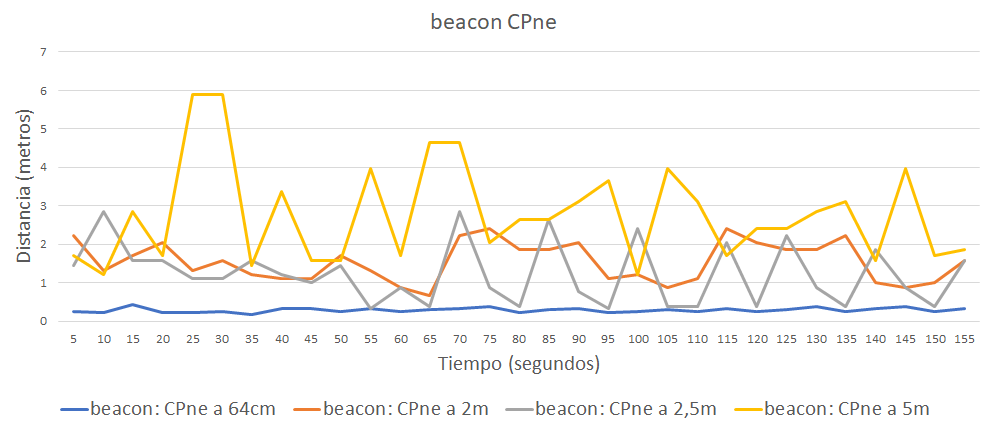
\includegraphics[width=0.7\textwidth]{Imagenes/Descripciondeltrabajo/dist_CPne}
	\caption{Gráfico con las distancias medidas al beacon CPne. }
	\label{fig:dist_CPne}
\end{figure}

En el caso de la Figura \ref{fig:dist_eAaw}, en la que se estima la distancia para el \textit{beacon} eAaw, el comportamiento es similar. En líneas generales, el valor medio estimado se corresponde con la distancia real a la que se encuentran las balizas. Sin embargo, en esta medición hemos contemplado una novedad que se ha repetido en numerosas ocasiones convirtiéndose en un patrón de comportamiento y es que durante los primeros segundos en los que arranca la aplicación, las estimaciones son menos precisas, dando lugar a picos importantes que más tarde se suavizan. 

La Figura \ref{fig:dist_8v2c} recoge cuatro mediciones para el \textit{beacon} 8v2c, tres de ellas tomadas para una misma distancia (4m) y una a 64 cm. Observamos de nuevo que el error es despreciable cuando la baliza se encuentra muy próxima. Por el contrario, los valores que recogen las gráficas en las que el dispositivo se encuentra a 4m están muy por debajo de lo esperado, solo una de ellas alcanza el valor real. Este factor común revela una alteración considerable de la intensidad de la señal provocada por algún factor del entorno que la debilita. Es por esto que la última gráfica plasmada en la Figura \ref{fig:dist_conjunto}, hace referencia a una situación particular. Se trata de dos \textit{beacons} diferentes situados a la misma distancia uno encima del otro. El objetivo de este estudio era ver si uno de los factores que podía alterar la intensidad de señal era la presencia de otras balizas, y efectivamente como podemos observar, la intensidad de ambas señales es bastante más baja de lo esperado, prácticamente en ningún momento alcanzan el valor real. En este caso particular, el error es tolerable ya que los \textit{beacons} están situados a muy poca distancia pero sí nos advierte de que la señal bluetooth es sensible a interferencias provocadas por otros \textit{beacons} del entorno. En el siguiente apartado estudiaremos qué otros posibles factores pueden ser los desencadenantes de alteraciones en la señal. 

Cabe destacar que aunque en determinados casos los datos son muy fluctuantes y poco precisos, las categorías de proximidad, con los rangos establecidos, se mantienen en su mayoría fieles a la realidad.


\begin{figure}[t]
	\centering
	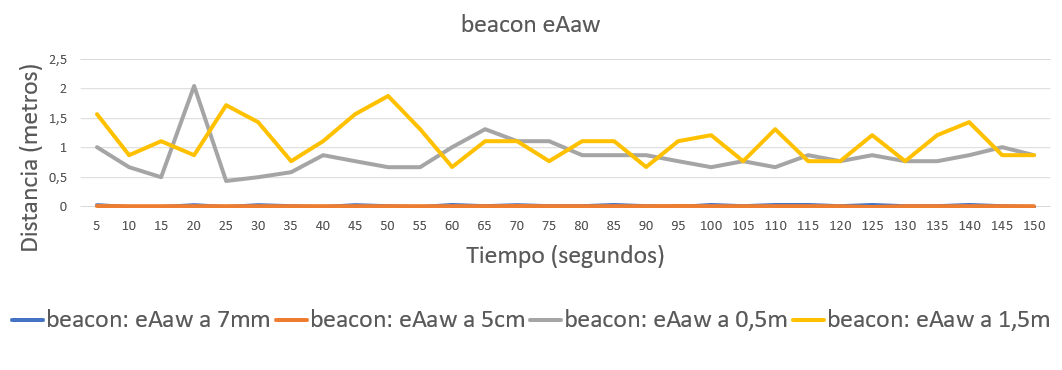
\includegraphics[width=0.7\textwidth]{Imagenes/Descripciondeltrabajo/dist_eAaw}
	\caption{Gráfico con las distancias medidas al beacon eAaw. }
	\label{fig:dist_eAaw}
\end{figure}


\begin{figure}[t]
	\centering
	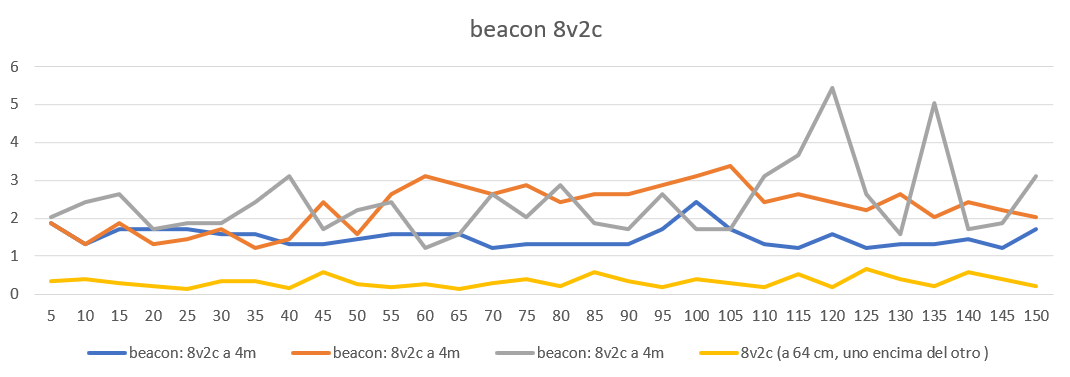
\includegraphics[width=0.7\textwidth]{Imagenes/Descripciondeltrabajo/dist_8v2c}
	\caption{Gráfico con las distancias medidas al beacon 8v2c. }
	\label{fig:dist_8v2c}
\end{figure}

\begin{figure}[t]
	\centering
	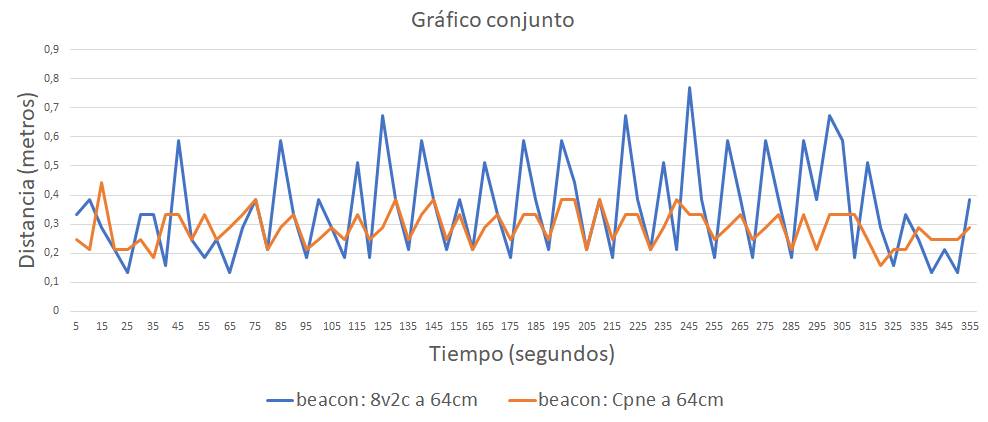
\includegraphics[width=0.7\textwidth]{Imagenes/Descripciondeltrabajo/dist_conjunto}
	\caption{Gráfico de los beacons 8v2c y CPne superpuestos. }
	\label{fig:dist_conjunto}
\end{figure}

\subsection{Interferencias en la señal bluetooth}

Los \textit{beacons} son dispositivos que se pueden colocar tanto en interiores como en exteriores pero hay que tener en cuenta qué lugares son más aptos para su establecimiento de manera que la señal no sufra interferencias, algunas recomendaciones son:
\begin{itemize}
	\item Lugares altos (alrededor de 2,5m) para evitar las interferencias provocadas por los cuerpos de las personas ya que estos absorben parte de la señal.
	\item Lugares alejados a un metro aproximadamente de elementos que pueden alterar la intensidad de la señal como elementos metálicos, conductos de electricidad, iluminación, otras balizas, etc.
	\item En pasillos de menos de 4m de ancho, colocar la baliza en el medio para que cubra el espacio por igual. Si por el contrario, el ancho es mayor se deberán usar varias balizas.
	\item Colocar las balizas aproximadamente 1m antes de los lugares de interés (\textit{landmarks}) en los que las personas necesitarán la siguiente instrucción. Ejemplo: puertas, ascensores, escaleras, esquinas, etc.
	\item Considerar la orientación adecuada de la antena direccional del \textit{beacon}, esta depende por completo del fabricante. En ocasiones la baliza no emite una señal simétrica por completo sino que emite una señal en forma elíptica.
\end{itemize}

Otros factores difíciles de controlar que también afectan a la señal son las condiciones meteorológicas, la señal Wi-Fi, las señales bluetooth de otros dispositivos...

%BIBLIOGRAFIA http://www.wayfindr.net/wp-content/uploads/2018/07/Wayfindr-Open-Standard-Rec-2.0.pdf?version=recommendation-2

\subsection{Mediciones en puntos clave de la facultad}
\label{sec:medicionesbeacons}

Ahora que hemos superado la primera barrera tecnológica y tenemos una idea más clara del funcionamiento y el comportamiento de los \textit{beacons}, nos disponemos a dar el siguiente paso hacia la resolución del problema del posicionamiento. Para ello, estudiaremos los planos de la Facultad de Informática, determinaremos cuales podrían ser, a priori, los puntos de decisión y haremos mediciones para comprobar si las señales de los \textit{beacons} se reciben correctamente y no sufren interferencias en dichos puntos.

Los puntos de decisión son aquellos lugares de interés para el usuario o aquellos puntos en los que se requerirá la siguiente instrucción a seguir en la ruta. Los puntos de decisión que hemos considerado son: los destinos (aulas, cafetería, biblioteca, conserjería, secretaría, salón de actos, sala de juntas, sala de grados, etc.), las intersecciones (esquinas), los ascensores y escaleras, y las puertas de entrada al edificio.

En las Figuras \ref{fig:medidasPBaja} y MEDIDASPLANTA1 mostramos visualmente algunos de los puntos en los que hemos probado a colocar los \textit{beacons} (puntos rojos) y desde donde hemos llevado a cabo las mediciones correspondientes (cruces verdes). El objetivo de este estudio es conocer la ubicación óptima de los \textit{beacons} para que a nuestro paso cerca de ellos, la distancia registrada sea lo más precisa posible, especialmente en los lugares más complicados como las intersecciones o las zonas en las que se acumulan varios puntos de interés (como el \textit{hall} de entrada). En el ANEXO se pueden ver los resultados de estas mediciones (HABRÁ QUE AÑADIR MÁS MEDICIONES-COMPLETAR). A continuación exponemos algunas de las conclusiones recogidas:

\begin{itemize}
	\item Los \textit{beacons} no deben situarse demasiado cerca ya que las señales interfieren entre sí y alteran las distancias no pudiendo distinguir cuál es el \textit{beacon} más cercano. Por este motivo, hemos acordado no poner, por el momento, balizas en los baños ya que, tanto en la planta 1 como en la planta baja, se encuentran en zonas repletas de puntos de interés.
	
	\item En lugares diáfanos, como el \textit{hall}, la señal de los \textit{beacons} fluye con mayor libertad ya que no se encuentra con obstáculos. Es por esto, que deben situarse a mayor distancia entre sí. Uno de los problemas que se ha derivado de este hecho es cómo cubrir dicho espacio. Inicialmente colocamos una baliza en conserjería, otra en la intersección superior con el pasillo principal, otra en la intersección inferior con el pasillo que conduce a cafetería y otra enfrente para indicar la entrada al salón de actos (ver Figura FIGURAMAPAPLANTABAJA). Tras numerosas mediciones, la solución que proponemos es colocar las balizas de modo que una pueda servir para cubrir dos o más puntos de interés. Consecuentemente, hemos suprimido el \textit{beacon} de conserjería y hemos dejado exclusivamente el de las intersecciones ya que la inferior está muy próxima a la ventanilla de conserjería y puede reutilizarse para los dos puntos clave, y hemos desplazado un poco hacia arriba el \textit{beacon} del salón de actos para que sirva tanto para marcar dicho destino como para marcar la esquina superior que conduce hacia la biblioteca. En la Figura FIGURANUEVA se puede ver el resultado final.
	
	\item Hemos hecho pruebas con los \textit{beacons} sobre distintas superficies y hemos comprobado que efectivamente el material puede alterar la señal. Particularmente, en el caso de las mediciones de la puerta lateral del edificio (lado izquierdo del mapa) hemos colocado el \textit{beacon} CPne justo encima de la puerta, en un bisel metálico que sobresale. El resultado ha sido que la señal de la baliza se proyecta con mayor intensidad, dando lugar a que la distancia estimada sea menor. Es decir, la aplicación sugiere que CPne está más cerca de lo que en realidad está. Tras esto, hemos concluido que lo óptimo es poner los \textit{beacons} sobre las mismas superficies, a ser posible no metálicas, y a la misma altura para que estén en igualdad de condiciones. 
	
	\item La última puntualización que hemos hecho tras las mediciones es que los \textit{beacons} de las intersecciones deben situarse en un punto lo más neutro posible ya que, al menos, se puede llegar desde dos puntos distintos y la señal se debe recibir de manera simétrica. 
\end{itemize}

\begin{figure}[t]
	\centering
	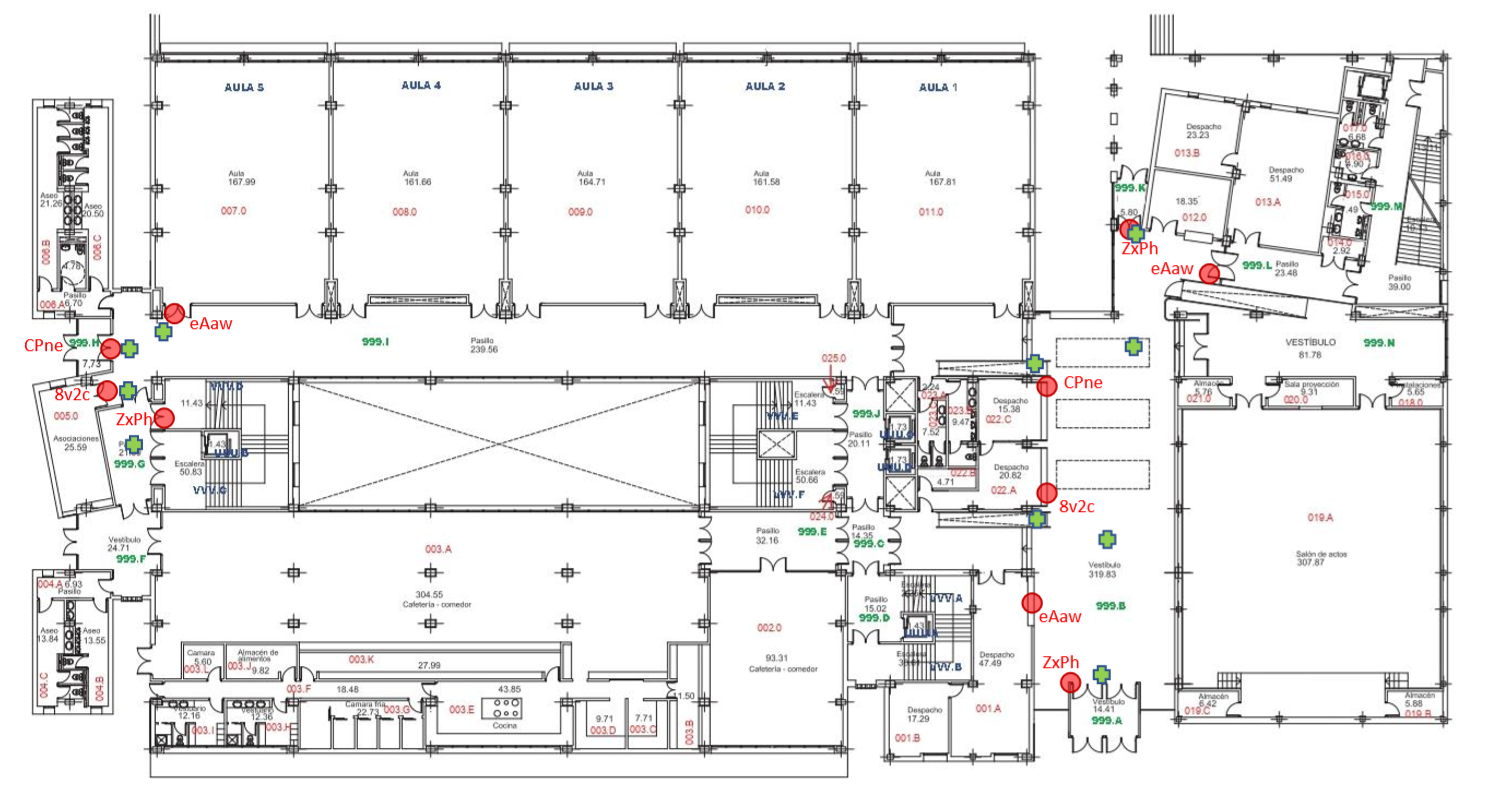
\includegraphics[width=1\textwidth]{Imagenes/Descripciondeltrabajo/medidasPlanoPBaja}
	\caption{Mapa de la planta baja de la Facultad de Informática con la ubicación de los beacons (rojo) y los puntos de medición (verde). }
	\label{fig:medidasPBaja}
\end{figure}

En la próxima sección veremos en qué se traducen todos estos resultados, cómo resulta la disposición final de los \textit{beacons} y cómo dividiremos los planos para llevar a cabo el mapeo del edificio.


\section{Mapeo del edificio}
\label{sec:mapeo}
Para el mapeo de la Facultad de Informática nos hemos apoyado en el proyecto \textit{Generador interactivo de instrucciones de guía sobre plataformas móviles} \citep{TFGguia}. De este, hemos reutilizado el sistema de estructuración basado en cuadrantes que contienen un identificador único (para diferenciar más fácilmente en qué planta estamos), y hemos prescindido de las posiciones sureste y noroeste ya que al emplear un sistema de posicionamiento basado en puntos de decisión no vamos a triangular la posición exacta del usuario y, por tanto, no necesitamos conocer las coordenadas (x,y) concretas de los cuadrantes. En su lugar hemos incluido el identificador (único) del \textit{beacon} asociado a dicho cuadrante. Por este mismo motivo, aquellos cuadrantes que no tienen asociada una baliza bluetooth carecen de interés ya que el programa te sitúa en el cuadrante con el \textit{beacon} más cercano desde tu posición. Es por esto que hemos aunado los cuadrantes formando unos nuevos más grandes. En la Figura \ref{fig:cuadrantesP1_v1} mostramos la planta 1 con los cuadrantes originales (en rojo) , su identificador (en verde) y la posición final de los \textit{beacons} (en amarillo) según lo que acordamos en la Sección \ref{sec:medicionesbeacons}, mientras que en la Figura \ref{fig:cuadrantesP1_v3} encontramos la versión final, en la que solo permanecen los cuadrantes con baliza. Además podemos observar que hemos suprimido los cuadrantes de las aulas, sala de juntas, etc. esto se debe a que nuestra aplicación no te guía dentro de estas estancias sino que funciona como guía de puerta a puerta.

\begin{figure}[t]
	\centering
	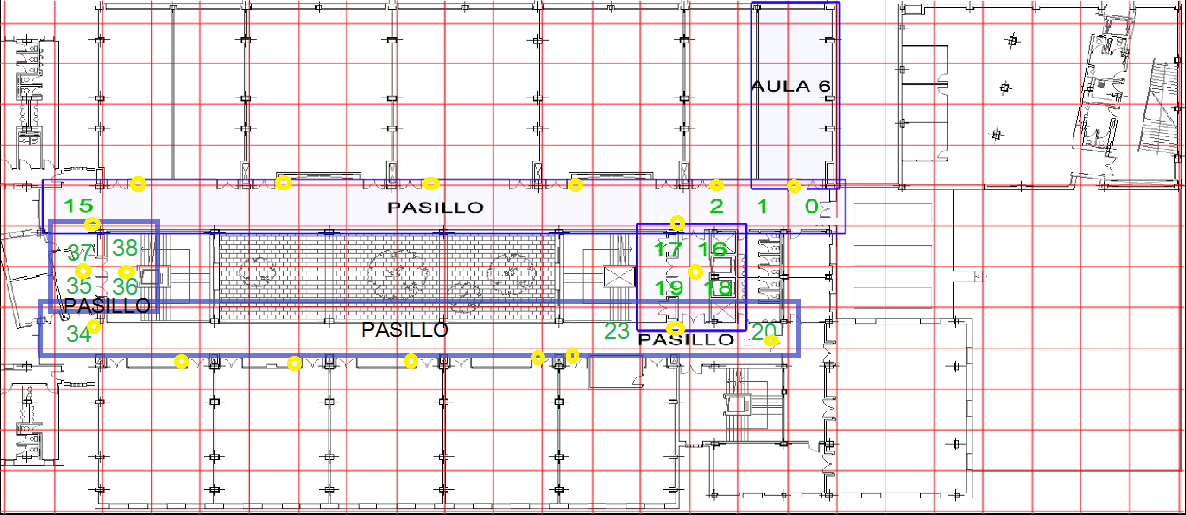
\includegraphics[width=1\textwidth]{Imagenes/Descripciondeltrabajo/mapaplanta1_cuadrantes}
	\caption{Primera versión del mapeo de la planta 1 de la Facultad de Informática.}
	\label{fig:cuadrantesP1_v1}
\end{figure}

\begin{figure}[t]
	\centering
	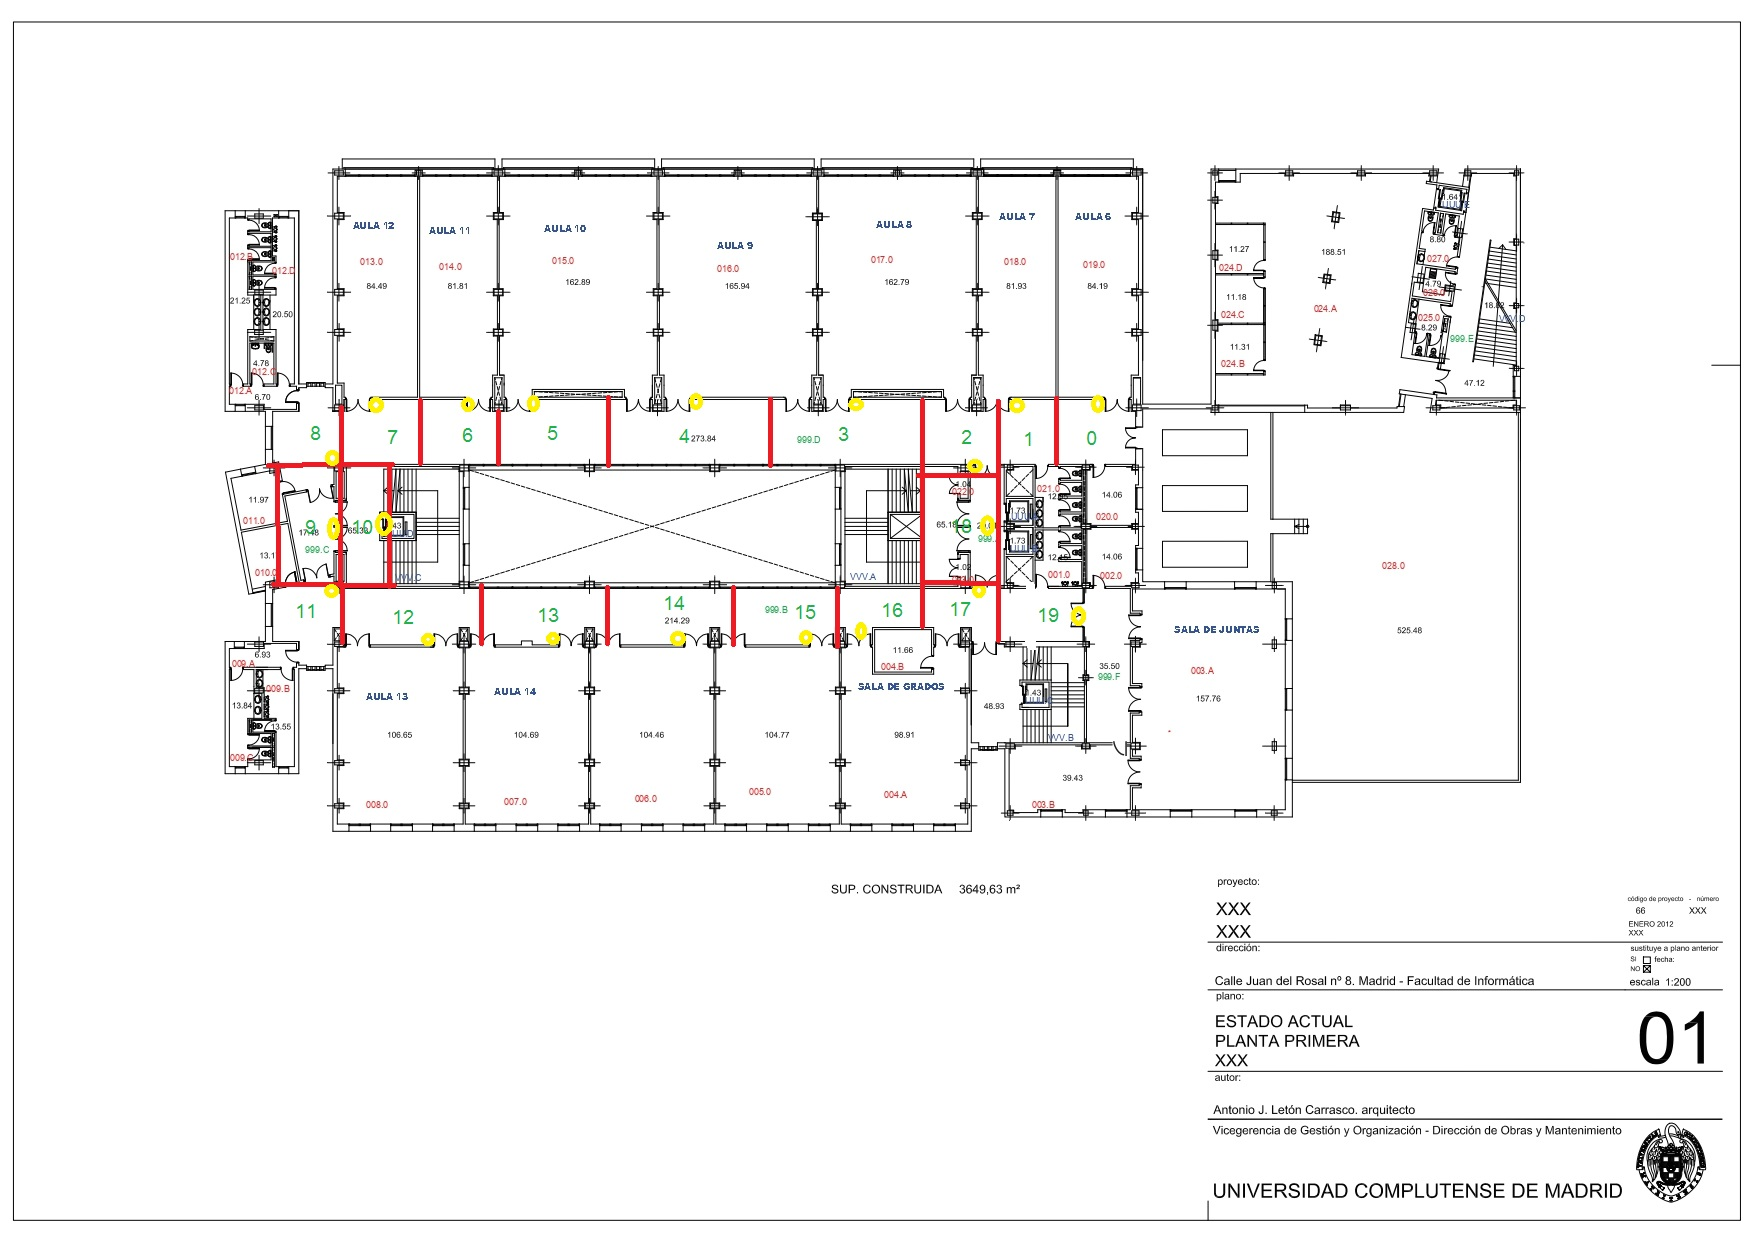
\includegraphics[width=1\textwidth]{Imagenes/Descripciondeltrabajo/mapaplanta1_cuadrantes3}
	\caption{Versión final del mapeo de la planta 1 de la Facultad de Informática.}
	\label{fig:cuadrantesP1_v3}
\end{figure}

Para poder establecer una red de cuadrantes que nos permita generar una ruta válida pasando a través de ellos, hemos mantenido la información de conectados con cada cuadrante por los puntos cardinales (norte, sur, este y oeste).

Esta estructura, junto con la información sobre la planta (coordenada z) en la que te encuentras, queda guardada en unos ficheros .xml almacenados en el servidor en una carpeta llamada xml\_modif que se encuentra en el mismo directorio de la aplicación compilada del servidor .jar. Estos ficheros son:

\begin{itemize}
	\item edificio.xml: Archivo principal, recuperado del proyecto mencionado, que indexa las diferentes plantas del edificio.
	\item plantaX.xml: Archivo que representa una planta del edificio.	
\end{itemize}

Otras novedades que hemos incluido en los archivos plantaX.xml son: añadir los metros que ocupan los cuadrantes para poder dar una instrucción más precisa, y añadir un apartado \textit{info} para poder informar al usuario, si lo desea, de qué hay a su paso por la ruta, esta idea la tuvimos tras investigar distintas aplicaciones de guía para personas con discapacidad visual y tras la reunión con la ONCE, en la que nos acercamos mucho a las necesidades de nuestros usuarios. Por otro lado, como podemos ver en la Figura \ref{fig:cuadrantesPbaja} hemos incluido el mapeo de la planta baja y hemos conectado las distintas plantas para incluir rutas de una a otra (novedad con respecto a los trabajos predecesores).

%HAY QUE CAMBIAR LA IMAGEN CUANDO CAMBIE EL CUADRANTE SIN BEACON!!
\begin{figure}[t]
	\centering
	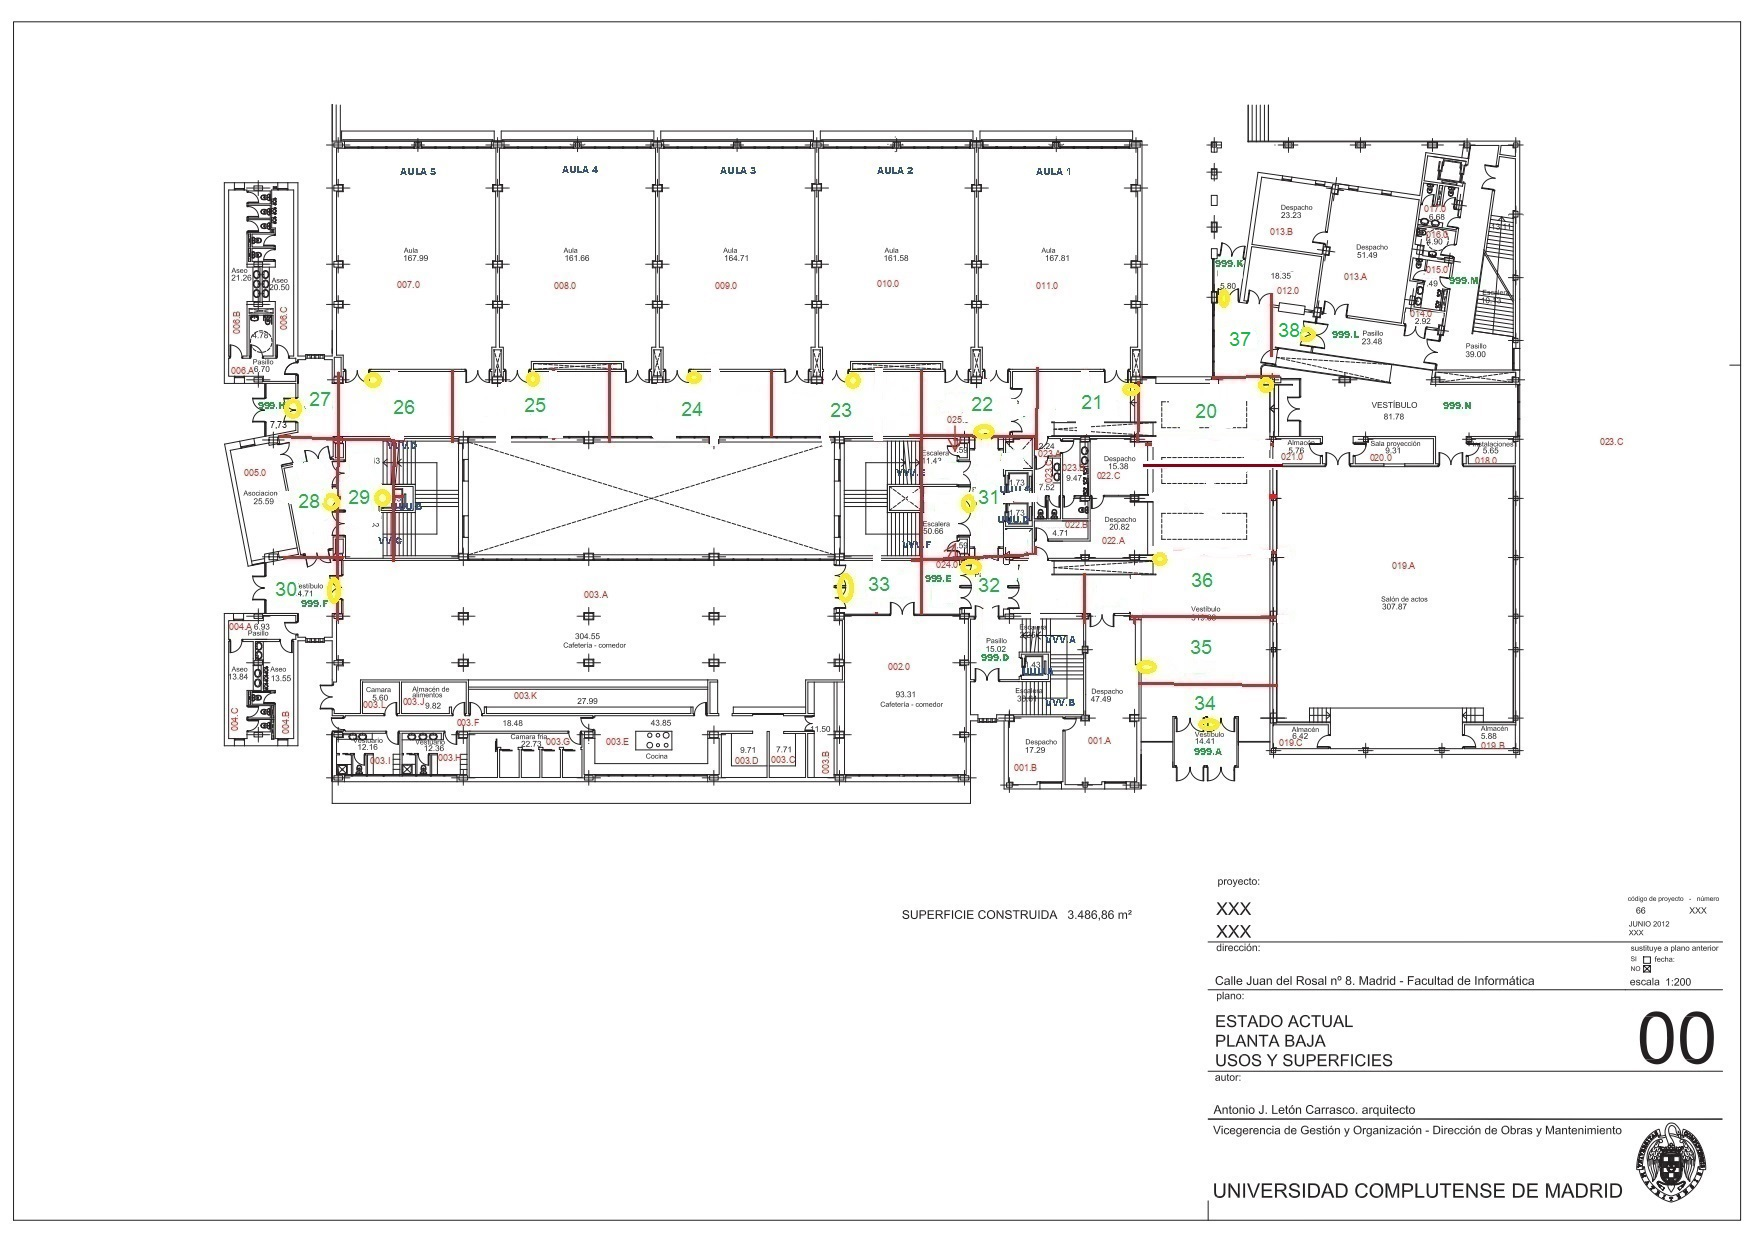
\includegraphics[width=1\textwidth]{Imagenes/Descripciondeltrabajo/mapaplantabaja_cuadrantes3}
	\caption{Mapeo de la planta baja de la Facultad de Informática.}
	\label{fig:cuadrantesPbaja}
\end{figure}

